\documentclass[numbers=noenddot,12pt,a4paper]{scrartcl}
\usepackage[greek,ngerman]{babel}
\usepackage[T1]{fontenc}
\usepackage[utf8]{inputenc}
\usepackage{ifoddpage}
\usepackage{libertine}
\usepackage{ziffer}
\usepackage{graphicx}
\usepackage{units}
\usepackage[infoshow]{tabularx}
\usepackage{amsmath}
\usepackage{fancyhdr}
\usepackage{amssymb}
\usepackage{wrapfig}
\usepackage{esint}
\usepackage{float}
\usepackage{wrapfig}
\usepackage[font=small]{caption}
\usepackage{subcaption}
\usepackage{lscape}
\usepackage{hyperref}

\renewcommand{\thefigure}{Abb. \arabic{figure}}

\captionsetup[wrapfigure]{name=}
\captionsetup[figure]{name=}
\newcommand{\degree}{^\circ}
\newcommand{\diff}{\textnormal{d}}
\newcommand{\tenpo}[1]{\cdot 10^{#1}}
\newcommand{\greek}[1]{\greektext#1\latintext}
\newcommand{\ix}[1]{_\text{#1}}
\newcommand{\imag}{\mathbf{i}}
\newcommand{\tilt}[1]{\textit{#1}}
\newcommand{\grad}[1]{\textit{grad}\left(#1\right)}
\newcommand{\divergenz}[1]{\textit{div}\left(#1\right)}
\newcommand{\euler}{\mathnormal{e}}
\newcommand{\fett}[1]{\textbf{#1}}
\newcommand{\wellenfunktion}{\Psi\left(\vec{r},t\right)}
\newcommand{\wellenfunktiont}{\Psi\left(\vec{r}\right)}
\newcommand{\winkel}{\text{Y}^{m}_{l}\left(\vartheta,\varphi\right)}
\newcommand{\radial}{\text{R}^{n}_{l}\left(r\right)}
\renewcommand{\headrulewidth}{0.1pt}
\renewcommand{\footrulewidth}{0.1pt}
\newcommand{\name}{\text{Philipp Hacker}} %TODO Name des Protokollanten eintragen

\title{Protokoll: Quantum Analogs} %TODO Name des Versuchs eintragen
\author{Tom Kranz, Philipp Hacker}
\date{\today}
\pagestyle{fancy}
\fancyhead[C]{\thepage}
\fancyhead[R]{\name}
\fancyfoot[C]{}
\fancyfoot[R]{\today}
\fancyhead[L]{Abschnitt \thesection}
\begin{document}
\maketitle
\begin{center}
Betreuer: S. Peglow \\ %TODO Name des Betreuers eintragen
Versuchsdatum: 12.11.2014 \\ %TODO Datum des Versuchs eintragen
\begin{table}[h]
\centering
Note: %TODO Gute Note erhalten :)
\begin{tabularx}{1.5cm}{|X|}
\hline \\ \\
\hline
\end{tabularx}
\end{table}
\end{center}
\vspace*{\fill}
\tableofcontents
\vfill
\newpage
\section{Einleitung}
In diesem Experiment geht es um die Modellierung und Analogie quantenmechanischer Phänomene der Wellennatur von, beispielsweise Elektronenzuständen des Wasserstoffs. Hierfür werden Schallwellen innerhalb einfacher geometrischer Objekte (Zylinder, un-/gekoppelte Sphäre) in Hinblick auf ihre Resonanzfrequenzen untersucht. Jedoch beschränkt man sich in diesem einfachen Versuch auf den Vergleich eines Teilchens (Elektron im Orbit) in einem unendlich Tiefen Potentialtopf mit stehenden Schallwellen. Weiterführenden quantenmechanische Untersuchungen und Analogien werden nicht betrachtet. Schließlich lassen sich aus diesem Experiment, welches sich nur Akustik und einfacher Geometrie bedient, mehr Informationen über Quantenzustände gewinnen, als durch irgendeine andere direkte Methodik.
\fancyfoot[L]{\textit{}}
\newpage
\fancyfoot[L]{}
\section{Physikalische Grundlagen}
\subsection{Analogie: quantenmech. Teilchen -- stehende Schallwellen}
Die physikalischen Zustände stehender Schallwellen und eines quantenmechanischen Teilchens, welches sich in einem unendlich tiefen Potentialtopf befindet, ähneln sich sehr. Deswegen werden im Folgenden Vergleiche zwischen beiden auf grundlegender Ebene gemacht.
\subsubsection{Teilchen im Potentialtopf}
Die \textit{Schrödinger-Differentialgleichung}$^{1}$ für ein Elektron der Energie $E=\hbar\omega$ in einem unendlich tiefen Potentialtopf $V\left(\vec{r}\right)$ lautet
\begin{align}
	\imag \hbar \frac{\partial}{\partial t}\Psi\left(\vec{r},t\right)=E\Psi\left(\vec{r},t\right)=&\left(-\frac{\hbar^2}{2 m_e}\Delta+V\left(\vec{r}\right)\right)\Psi\left(\vec{r},t\right) \nonumber \\ 
	=&-\frac{\hbar^2}{2 m_e}\Psi\left(\vec{r},t\right) \label{eq:schrödinger}
	\end{align}
Die Wellenfunktion $\Psi\left(\vec{r},t\right)$ beschreibt im Allgemeinen die komplexe Wellenfunktion des Teilchens am Ort $\vec{r}$ zur Zeit $t$. Das absolute Betragsquadrat dessen spiegelt die Zustandsdichte und somit eine Aufenthaltswahrscheinlichkeit wider. \\
In (\ref{eq:schrödinger}) wurde die Differentialgleichung für das Innere des Topfes hingeschrieben. An den Ränder und außerhalb verlangen die Randbedingungen$^{2}$, dass dort die $\Psi\left(\vec{r},t\right)$ verschwindet. Außerdem nehmen wir an, dass die Lösung unseres Problems zeitunabhängig ist. Dies drückt die Ladungs- bzw. Energieerhaltung des Zustandes aus.\\
Nimmt man sich nun eine harmonische Lösung der Differentialgleichung (\ref{eq:schrödinger}) her und wendet darauf notwendige Normierungsbedingungen an, so erhält man
\begin{align}
	\Psi\left(\vec{r},t\right)=\sqrt{\frac{2}{a}}\sin\left(\vec{k}\vec{r}+\varphi_0\right)\cdot\euler^{-\imag\omega t} \, . \label{eq:lösung}
\end{align}
Hierbei ist $\vec{k}$ der Wellenzahlvektor, welcher in Ausbreitungsrichtung zeigt und für den gilt $|\vec{k}|=k=\frac{n\pi}{a}$ mit $n\in\mathbb{Z}$. Außerdem sei $a$ die Breite des Potentialtopfes und $\euler^{-\imag\omega t}$ ein einfacher Phasenfaktor, welcher $|\wellenfunktion|^2$ invariant lässt.\\
Geht man mit (\ref{eq:lösung}) zurück in (\ref{eq:schrödinger}), so findet man die Dispersionsrelation (\ref{eq:dispers}) des Teilchens.
\begin{align}
	E\left(k\right)=\frac{\hbar^2 k^2}{2m_e}=\frac{\hbar^2n^2\pi^2}{2m_e a^2} \label{eq:dispers}
\end{align}
\subsubsection{Stehende Schallwellen}
Eine Schallwelle kann als die Ausbreitung einer mechanischen Deformation eines Mediums verstanden werden. Sie ist immer eine Longitudinalwelle und genügt der Gleichung
\begin{align}
\Delta u=\frac{1}{c^2}\frac{\partial^2 u}{\partial t^2} \, \label{eq:welle}
\end{align}
Die Lösungen von (\ref{eq:welle}) können immer$^3$ durch die Linearkombination von trigonometrischen Funktionen dargestellt werden.

\fancyfoot[L]{$^{1}$ \textit{Begründer der Quantenmechanik, Erwin Schrödinger (1887-1961) \\
	$^{2}$ \text{Dirichlet-Randbedingungen} \\
	$m_e$ - Elektronenmasse; $\hbar$ - reduzierte Planck-Konstante; $\Delta$ - Laplace-Operator \\
	$c$ - Lichtgeschwindigkeit im Medium; $\omega$ - Kreisfrequenz}}
\newpage
\fancyfoot[L]{}

Sie haben die folgende Form:
\begin{align}
	u(\vec{r},t)=A\sin\left(\vec{r}\vec{k}-\omega t+\varphi_0\right) \, .\label{eq:wellenlösung}
\end{align}
Diese Wellen werden als laufend bezeichnet, da sie der Form $u\left(\vec{r}-\vec{v}\ix{Ph}t\right)$ genügen.\\
Allgemein können die Lösungen von (\ref{eq:welle}) als  $u\left(\vec{r},t\right)=f\left(\vec{r}+\vec{v}\ix{Ph}t\right)+g\left(\vec{r}-\vec{v}\ix{Ph}t\right)$, mit den 2-mal stetig differenzierbaren Funktionen $f$ und $g$, aufgefasst werden. Offensichtlich bewegt sich hier $f$ mit der Geschwindigkeit $\vec{v}\ix{Ph}$ vorwärts und $g$ entgegengesetzt.\\
Die Summe $\tilde{u}$ zweier Lösungen (\ref{eq:wellenlösung}) ist keine laufende Welle, da sie nicht mehr die Form $\tilde{u}\left(\vec{r}\pm\vec{v}\ix{Ph}t\right)$ hat:
\begin{align}
	\tilde{u}\left(\vec{r},t\right)=2A\cos\left(\vec{r}\vec{k}+\frac{\varphi_0}{2}\right)\cos\left(\omega t-\frac{\varphi_0}{2}\right) \, . \label{eq:stehend}
\end{align}
\begin{figure}[H]
	\centering
	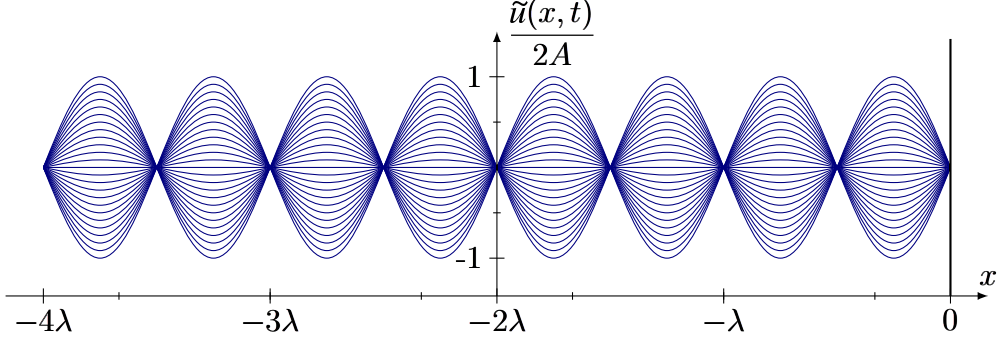
\includegraphics[width=\textwidth]{stehendewelle.png}
	\caption{Summe zweier laufenden Wellen in einem sogenannten Resonator (hartes Medium$^4$)} \label{img:stehendewelle}
\end{figure}
Sie heißt stehende Welle (siehe \ref{img:stehendewelle}). Für einen harten$^4$ Zylinder der Länge $L$ stellen sich stehende Wellen aus (\ref{eq:wellenlösung}) der Frequenz $f$ bzw. Wellenlänge $\lambda$ unter der Erfüllung der Bedingung
\begin{align}
n\frac{\lambda}{2}=n\frac{c}{2f}=n\frac{\pi c}{\omega}=L \label{eq:resonanz}
\end{align}
ein. Die ursprüngliche und die an den Wänden des Objektes reflektierte Welle befinden sich in gleicher Phase und addieren damit ihre Amplituden. Die Frequenz, bei welcher (\ref{eq:resonanz}) erfüllt ist, heißt auch Resonanzfrequenz.

\subsubsection{Vergleich}
Das wichtigste Analogon dieses Versuches ist das der Frequenzniveaus (bei Resonanzen) des Schallexperiments und der Energieniveaus der Elektronenzustände. Diese sind gerade die Eigenzustände der jeweiligen Systeme und lassen sich aus den Dispersionsrelationen $E\left(k\right)$ und $w\left(k\right)$ ableiten.\\

\fancyfoot[L]{$^3$ \textit{laut der Theorie der Fourier-Transformation\\
		$^4$ die Art des Mediums, an welcher die Wellen reflektieren, bestimmt den Phasensprung der zurückgeworfenen im Vergleich zur ursprünglichen\\
		$v\ix{Ph}$ - Phasengeschwindigkeit der Welle}}
\newpage
\fancyfoot[L]{}

Beide Differentialgleichungen (\ref{eq:schrödinger}) und (\ref{eq:welle}) beschreiben delokalisierte Objekte$^5$. Jedoch unterscheiden sie sich essentiell in ihrem Zeitdifferential. Die linke Seite der Gleichung (\ref{eq:schrödinger}) verlangt komplexe Lösungen, woraus die quadratische Dispersionsrelation (\ref{eq:dispers}) folgt. Der Einfluss eines Potentials $V\left(\vec{r}\right)$ in der Wellengleichung fehlt vollständig, wobei dennoch die harten Wände des Resonators in diesem Fall die Wellenfunktionen auf den Innenraum beschränken und somit ähnliche Randbedingungen wie für (\ref{eq:schrödinger}) fordern. Andererseits liegen die Knoten der Wellen an unterschiedlichen Stellen, da die Randbedingungen nicht die selben sind. Weiterhin kann durch eine Messung eines quantenmechanischen Zustandes $\wellenfunktion$ nur eine Aussage über die Aufenthaltswahrscheinlichkeit gemacht werden, wohingegen ein Mikrofon sowohl Phase und  Amplitude bei einer Schallwelle messen kann.

\subsection{Modellierung im sphärischen Resonator}
\subsubsection{Quantenmechanik} \label{subsec:wasserstoff}
Die analytische Lösbarkeit des Wasserstoffatom-Problems in der Quantenmechanik eignet sich äußerst gut für die Untersuchung durch eine akustisches Analogon mithilfe eines sphärischen Resonators. Das einfache, nicht durch Wechselwirkungen gestörte Elektron bewegt sich im Coulomb-Feld um den Kern. Gleichung (\ref{eq:schrödinger}) wird damit, unter Verwendung von Kugelkoordinaten, zur Gleichung (\ref{eq:schrödingerkugel}).
\begin{align}
	E\Psi\left(\vec{r}\right)=&\left(-\frac{\hbar^2}{2 m_e}\Delta-\frac{e^2}{r}\right)\Psi\left(\vec{r}\right) \nonumber \\
	=&\frac{\hbar}{2m_e r^2}\left(\frac{\partial}{\partial r}\left(r^2\frac{\partial}{\partial r}\right)+\frac{1}{\sin\left(\vartheta\right)}\left(\sin\left(\vartheta\right)\frac{\partial}{\partial \vartheta}\right)+\frac{1}{\sin^2\left(\vartheta\right)}\frac{\partial^2}{\partial \varphi^2} -\frac{e^2}{r}\right)\wellenfunktiont  \label{eq:schrödingerkugel} 
	\end{align}
Macht man einen Seperationsansatz für $\wellenfunktiont$ mit $\winkel$ und $\radial$, so erhält man die Kugelflächenfunktionen (\ref{eq:kff}) aus der Lösung der Winkelgleichung (\ref{eq:wwf}).
\begin{align}
	E^{n}\radial=&-\frac{\hbar}{2m_e r^2}\left(\frac{\partial^2}{\partial r^2}r -l\left(l+1\right)-\frac{e^2}{r}\right)\radial \label{eq:radi} \\ l\left(l+1\right)\hbar^2\winkel=&-\left(\frac{1}{\sin\left(\vartheta\right)}\left(\sin\left(\vartheta\right)\frac{\partial}{\partial \vartheta}\right)+\frac{1}{\sin^2\left(\vartheta\right)}\frac{\partial^2}{\partial \varphi^2}\right)\winkel \label{eq:wwf} \\
	\winkel=&\frac{1}{\sqrt{2\pi}}\sqrt{\frac{2l+1}{2}\frac{\left(l-1\right)!}{\left(l+1\right)!}}\text{P}^{l}\ix{m}\left(\cos\left(\vartheta\right)\right)\euler^{\imag m\varphi} \label{eq:kff}
\end{align}
\subsubsection{Akustik}
Für den Vergleich von Wasserstoffatomzuständen und stehenden Wellen nimmt man einen sphärischen Resonator her, welcher aufgrund seiner Symmetrien eine ähnliche theoretische Behandlung wie das Elektron um den Kern verlangt.\\
Schreibt man die Gleichung (\ref{eq:welle}) für den Druck auf und benutzt $p\left(\vec{r},t\right)=p\left(\vec{r}\right)\cos\left(\omega t\right)$, so erhält man die zeitunabhängige Helmholtzgleichung (\ref{eq:helm}).
\begin{align}
	-\frac{\omega^2}{c^2} p\left(\vec{r}\right)=\Delta p\left(\vec{r}\right) \label{eq:helm}
\end{align}

\fancyfoot[L]{\textit{$^5$ siehe: Welle-Teilchen-Dualismus\\
		$r$ - Bahnradius; $e$ - Elementarladung\\
		n,l,m - Haupt-, Drehimpuls- und Magnetquantenzahlen der Zustände}\\
	$\text{P}^{l}\ix{m}\left(x\right)$ - \textit{Legendre-Polynome}}
\newpage
\fancyfoot[L]{}

Verfährt man nun wie für das Wasserstoffatom in \ref{subsec:wasserstoff} weiter(Kugelkoordinaten usw.), so erkennt man, dass sich die selben Lösungen $\winkel$ für den Winkelanteil ergeben.\\
Letztlich ist es notwendig, sich gesondert die Radialgleichung für den akustischen Fall anzuschauen.
\begin{align}
	\left(-\frac{\partial^2}{\partial r^2}-\frac{2}{r}\frac{\partial}{\partial r}+\frac{l\left(l+1\right)}{r^2}\right)f\left(r\right)=\frac{\omega_{n}^2}{c^2}f\left(r\right) \label{eq:akustikrad}
\end{align}
\subsubsection{Vergleich}
Wie bereits erwähnt, erhält man die selben Winkellösungen $\winkel$ für die Zustände stehender Wellen im sphärischen Resonator und das Elektron um den Wasserstoffatomkern.\\
Das Coulomb-Potential ruft eine $n$-Fache Entartung des Wasserstoffzustandes hervor. Einem Wert $E$ genügen damit $n$ verschiedene Zustände. Für eine Kombination von $n$ und $l$ liegt daher in beiden Fällen eine $\left(2l+1\right)$-fache Entartung vor.\\
Da Gleichung $(\ref{eq:akustikrad})$ und $(\ref{eq:radi})$ verschiedene Formen haben, können Energie- und Frequenzniveaus $E^n$ und $\omega_n$ nur nach ihren Quantenzahlen verglichen werden. Schließlich ist im sphärisch-symmetrischen Resonator die einzige Resonanzfrequenz, welche nicht verschwindet, die mit $m=0$. Für diese hat $\winkel$ keine azimutale $\varphi$-Abhängigkeit. Daher genügt eine Beschränkung auf die Untersuchung von Werten für $l$.\\
Durch die Zerstörung der Symmetrie des Aufbaus verändern sich die Quantisierungsachse und damit auch die Entartungen. Folglich kann nicht mehr angenommen werden, dass die z-Achse auch die Symmetrieachse des Systems ist.\\
Es können somit Magnetquantenzahlzustände angeregt werden, für die ein jeweiliges $\pm m$ einer um die Quantisierungsachse rechts- bzw. linksdrehenden Welle gleicher Amplitude entspricht. Die Kombination von beiden ergibt die stehende Welle der betrachteten Resonanzfrequenz.
\begin{align}
\euler^{\imag m\varphi}+\euler^{\imag (-m) \varphi}=2\cos\left(m\varphi\right) \nonumber
\end{align}
\subsection{Molekülmodellierung}
Versteht man das Aneinanderfügen von 2 sphärischen Resonatoren als die Kombination von Atomorbitalen, so lässt sich mittels akustischer Resonanz das Verhalten von Molekülzuständen unter unterschiedlichen Kopplungstärken nachvollziehen.\\
Nimmt man einen großen Kernabstand an, so kann die Superposition der Elektronenzustände unter Näherung genutzt werden. Da homonukleare, zweiatomige Moleküle eine Zylindersymmetrie besitzen, ist die Magnetquantenzahl ein gutes Mittel zur Beschreibung von nicht-/bindenden Orbitalen. Bindende Molekülorbits haben große Energien und beherbergen Elektronen zwischen den Kernen. Nichtbindende Zustände schwächt jedoch die Aufnahme von Elektronen.\\
In diesem Versuch bestimmt eine Blende zwischen den Sphären die Kopplungsstärke (Abstand der Atome). Die selben Symmetrien bestehen und können von den gleichen Quantenzahlen beschrieben werden.
\section{Durchführung}
Eingangs wird an einem Metallzylinder (siehe \ref{img:quantum}) mit integriertem Lautsprecher der Frequenzgang der Resonanz verfolgt. Die Beobachtungen werden über ein Mikrofon, welches den Zylinder abschließt, und ein digitales Oszilloskop realisiert. Außerdem nutzten wir einen Frequenzgenerator und einen proprietären Wandler (siehe \ref{img:quantum}) für das Abgreifen der Signale. Die Länge des Objektes wird dabei variiert. Anschließend wird die bereitgestellte Software genutzt, um selbige Untersuchung zu wiederholen und mit der ersten Messung zu vergleichen.\\
Im zweiten Versuchsteil wird der besprochene sphärische Resonator aus zwei Metallhalbkugeln mit eingelassenem Mikrofon und Lautsprecher eingesetzt. An ihnen ist ein Winkelmaß aufgetragen, welche Aufschluss über den Schnittwinkel von Mikrofon- und Lautsprecherachse gibt (hierbei bedeutet dass Gegenüberliegen $\alpha=0^\circ$). Beachtet werden muss das Verhältnis von theoretischem und gemessenem Winkel:
\begin{align*}
	\cos\left(\vartheta\right)=\frac{1}{2}\cos\left(\alpha\right)-\frac{1}{2} \, .
\end{align*}
Wiederum wurde das Computerprogramm genutzt um ein größeres Frequenzspektrum aufzunehmen. Diese Messung wurde für 2 gegenüberliegende Winkel unternommen.\\
Es schloss sich eine detailliertere Messung eines eingeschränkten Frequenzbereiches unter kleiner Veränderung des Winkel an. Für den einfachen sphärischen Resonator betrachteten wir schließlich polare Plots, dh. eine von der gestellten Software erzeugte Visualisierung des Atomorbitals unter sukzessiver Änderung des Winkels $\alpha$.\\
Im letzten Teil koppelten wir für verschiedene Blendenstärken ($\unit[5-15]{mm}$) zwei Resonatorsphären miteinander. Dabei Verglichen wir in einem kleinen Frequenzbereich die Resonanzfrequenzen des einzelnen Atoms mit denen unterschiedlich stark gekoppelter. Im Abschluss betrachteten wir nochmals das Bild der Wellenfunktion für die stärkste Kopplung beider Atomorbitale.


\begin{figure}[H]
	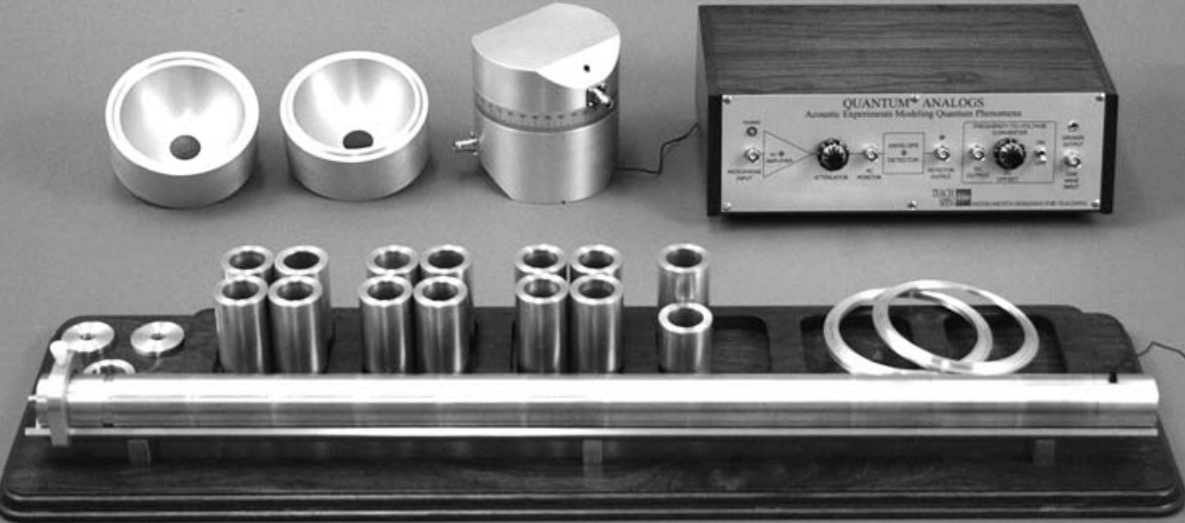
\includegraphics[width=0.9\textwidth]{quatumsw1.png}
	\centering
	\caption{Vordergrund: Zylinderaufbau; Hintergrund: v.l.n.r einfache und gekoppelte Sphären, Wandler} \label{img:quantum}
\end{figure}

\fancyfoot[L]{\textit{}}
\newpage
\fancyfoot[L]{}

\section{Auswertung}


\fancyfoot[L]{\textit{}}
\newpage
\fancyfoot[L]{}

\section{Anhang}
\section{Quellen}
\begin{itemize}
	\item{\url{http://ephex.phys.ethz.ch/fileadmin/user_upload/Experimente/Versuchsbeschrieb/05-06-07%20Stehende%20Schallwellen.pdf}\\ S.3, Gl. (2)-(4); Abb. 4}
	\item{\url{http://de.wikipedia.org/wiki/Wellengleichung#L.C3.B6sungen_der_homogenen_Wellengleichung_in_einer_r.C3.A4umlichen_Dimension}\\ Abschn.: "`Lösungen der homogenen Wellengleichung in einer räumlichen Dimension"'}
	\item{\url{http://www.teachspin.com/newsletters/TeachSpin_FEB08.pdf}\\ S.1, \ref{img:quantum}}
\end{itemize}
\end{document}